\chapter{Introduction}

Time management has become increasingly complex in our interconnected world, where individuals juggle multiple calendars, commitments, and communication channels. This chapter introduces Jadwal, an intelligent iOS-based calendar management system designed to address these modern challenges. We will explore the background, objectives, scope, and significance of this project, highlighting how it aims to revolutionize personal time management through intelligent automation and integration with communication platforms.


\section{Background of the Project}

Calendars have been around a long time now, and they are a handy tool for humans. Both who are busy and who want to plan their days. People throughout history have used paper for calendars, but now with technology, things have changed. Calendars are digital now, and they can even be shared with others!

As the world is becoming one big village with globalization, people tend to squeeze every last minute of their days since competition is higher. Calendars help in that since they allow people to plan their days easily and keep track of when to meet people and do other activities.

People these days use multiple calendars and sometimes forget to insert an event to the correct calendar.

\section{Problem Statement}

Keeping your calendar up to date with event information is challenging, especially with the rise of many informal communication channels like WhatsApp. People nowadays discuss when and where they will meet using those informal communication tools. This leads to calendars being out of sync from real life events you are committed to and might harm relations. The problem lies in the cumbersomeness of adding events to a calendar manually. And when people are busy, they just forget that they didn't add the event to their calendar. Our Jadwal app aims to solve this issue for users in an intelligent way that makes it seamless to manage your time confidently.

\section{Objectives of the Project}

The development of Jadwal is driven by clear, measurable objectives that address the current challenges in calendar management. These objectives focus on creating an intelligent system that seamlessly integrates multiple calendars, automates event extraction, and prioritizes user efficiency while maintaining prayer schedules. Each objective has been carefully defined to ensure the final product delivers meaningful value to users.

The main objectives of Jadwal are:
\begin{itemize}

    \item To integrate all the calendars into Jadwal's single calendar view to make viewing and managing all the events easy.
    \item To develop an intelligent calendar management system that automatically extracts events from the informal communication channels like WhatsApp and adds them to the user's main calendar.
    \item To significantly reduce the time users spend on manual calendar management.
    \item To create a user friendly interface that allows users to easily add events to the calendar.
    \item To prioritize and automatically schedule daily routines such as prayer time.
    \item To implement a smart resolution system that notifies users of scheduling conflicts and provides easy options for resolution.
\end{itemize}

\section{Scope of the Project}

Jadwal is not just another calendar application; it's a comprehensive time management tool designed to aggregate and optimize your existing calendars and data sources. The scope of the project includes:
\begin{itemize}
    \item Development of an iOS application as the primary platform.
    \item Integration with calendars using CalDAV.
    \item WhatsApp message parsing for event extraction using state-of-the-art LLMs (subject to technical feasibility).
    \item Target audience: Busy professionals, students, and anyone juggling multiple schedules.
    \item User testing phase to ensure ease of use and effectiveness. Our testing methods will include:
          \begin{itemize}
              \item Beta testing with a diverse group of users.
              \item Analytics to track user behavior and app performance.
          \end{itemize}
\end{itemize}


\section{Significance of the Project}

In today's fast-paced environment, effective time management is not just a convenience—it's a necessity. Jadwal addresses critical gaps in existing calendar solutions by introducing innovative features that align with modern users' needs. The project's significance extends beyond simple calendar management, offering transformative benefits for personal productivity, religious observance, and professional organization. By tackling the challenges of fragmented schedules and missed commitments, Jadwal represents a significant advancement in how people manage their time in the digital age.

Jadwal's significance can be summarized in the following points:
\begin{enumerate}
    \item \textbf{Time is Money}: Since time is the only asset you can't get more of, Jadwal tries to make it less painful and less time consuming to have a good calendar throughout your day by parsing events from your informal communication channels like WhatsApp automatically.
    \item \textbf{Prayer First Calendar}: Prayer times come first, then your daily scheduled items.
    \item \textbf{Reduced Human Error}: Automated event extraction and addition to calendars minimize the risk of missing important events or appointments due to manual input errors or forgetfulness.
    \item \textbf{Conflict Resolution}: The smart resolution system helps users identify and resolve scheduling conflicts efficiently, reducing stress and improving overall time management.
    \item \textbf{Holistic View of Commitments}: By integrating multiple calendars into a single view, Jadwal provides users with a comprehensive overview of their commitments across various aspects of life, facilitating better decision-making and work-life balance.
\end{enumerate}

\section{Limitations of the Project}

While Jadwal introduces innovative solutions to calendar management, it is essential to acknowledge and understand its current constraints and limitations. These limitations stem from various factors including technological boundaries, privacy concerns, third-party dependencies, and resource constraints. By identifying these limitations early in the development process, we can better manage user expectations and plan future improvements to address these challenges.

Nothing is perfect, and our project is not an outlier. The limitations we have figured out about it are as follows:
\begin{itemize}
    \item WhatsApp integration allows the app to read the user's messages, so it would be difficult to prove that privacy hasn't been breached.
    \item WhatsApp integration might not always be there, they are a third-party.
    \item Learning new technologies for iOS development might require more time than anticipated.
    \item Accuracy of our algorithms to detect keywords indicating an event agreement has happened, especially for languages other than English.
    \item Time and manpower constraints may limit the number of features we can implement.
    \item Dependency on third-party APIs and their limitations.
    \item We may face a challenges to test the app due to lack of users for testing our app
\end{itemize}

\section{Organization of the Senior Project}

To ensure systematic development and timely delivery of Jadwal, we have established a detailed project timeline with clear milestones and deliverables. The Gantt chart, shown in \textbf{Figure~\ref{fig:project-gantt-chart}}, illustrates our project's phases, tasks, and their respective durations.

\begin{figure}[!h]
    \centering
    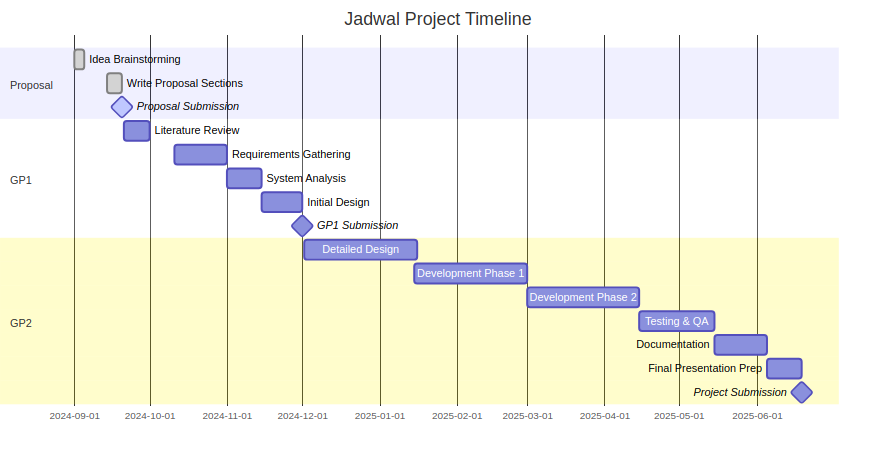
\includegraphics[width=\textwidth]{images/gantt.png}
    \caption{Project Gantt Chart}
    \label{fig:project-gantt-chart}
\end{figure}

\section{Conclusion}

In conclusion, the shift from traditional calendars to digital ones has changed how people organize their schedule.
While digital calendars offer easy and conflict free scheduling which makes managing easy.
Discussion on informal communication channels like WhatsApp has impacted the planning events and commitments.
This impact often leads to missed appointments and scheduling conflicts, especially for someone who is busy.

Jadwal aims to solve this issue by providing a seamless and automated solution for integrating informal communication with the application so that no one misses an event or have conflicts.

\cleardoublepage